% Options for packages loaded elsewhere
\PassOptionsToPackage{unicode}{hyperref}
\PassOptionsToPackage{hyphens}{url}
\PassOptionsToPackage{dvipsnames,svgnames,x11names}{xcolor}
%
\documentclass[
  letterpaper,
  DIV=11,
  numbers=noendperiod]{scrartcl}

\usepackage{amsmath,amssymb}
\usepackage{lmodern}
\usepackage{iftex}
\ifPDFTeX
  \usepackage[T1]{fontenc}
  \usepackage[utf8]{inputenc}
  \usepackage{textcomp} % provide euro and other symbols
\else % if luatex or xetex
  \usepackage{unicode-math}
  \defaultfontfeatures{Scale=MatchLowercase}
  \defaultfontfeatures[\rmfamily]{Ligatures=TeX,Scale=1}
\fi
% Use upquote if available, for straight quotes in verbatim environments
\IfFileExists{upquote.sty}{\usepackage{upquote}}{}
\IfFileExists{microtype.sty}{% use microtype if available
  \usepackage[]{microtype}
  \UseMicrotypeSet[protrusion]{basicmath} % disable protrusion for tt fonts
}{}
\makeatletter
\@ifundefined{KOMAClassName}{% if non-KOMA class
  \IfFileExists{parskip.sty}{%
    \usepackage{parskip}
  }{% else
    \setlength{\parindent}{0pt}
    \setlength{\parskip}{6pt plus 2pt minus 1pt}}
}{% if KOMA class
  \KOMAoptions{parskip=half}}
\makeatother
\usepackage{xcolor}
\setlength{\emergencystretch}{3em} % prevent overfull lines
\setcounter{secnumdepth}{-\maxdimen} % remove section numbering
% Make \paragraph and \subparagraph free-standing
\ifx\paragraph\undefined\else
  \let\oldparagraph\paragraph
  \renewcommand{\paragraph}[1]{\oldparagraph{#1}\mbox{}}
\fi
\ifx\subparagraph\undefined\else
  \let\oldsubparagraph\subparagraph
  \renewcommand{\subparagraph}[1]{\oldsubparagraph{#1}\mbox{}}
\fi

\usepackage{color}
\usepackage{fancyvrb}
\newcommand{\VerbBar}{|}
\newcommand{\VERB}{\Verb[commandchars=\\\{\}]}
\DefineVerbatimEnvironment{Highlighting}{Verbatim}{commandchars=\\\{\}}
% Add ',fontsize=\small' for more characters per line
\usepackage{framed}
\definecolor{shadecolor}{RGB}{241,243,245}
\newenvironment{Shaded}{\begin{snugshade}}{\end{snugshade}}
\newcommand{\AlertTok}[1]{\textcolor[rgb]{0.68,0.00,0.00}{#1}}
\newcommand{\AnnotationTok}[1]{\textcolor[rgb]{0.37,0.37,0.37}{#1}}
\newcommand{\AttributeTok}[1]{\textcolor[rgb]{0.40,0.45,0.13}{#1}}
\newcommand{\BaseNTok}[1]{\textcolor[rgb]{0.68,0.00,0.00}{#1}}
\newcommand{\BuiltInTok}[1]{\textcolor[rgb]{0.00,0.23,0.31}{#1}}
\newcommand{\CharTok}[1]{\textcolor[rgb]{0.13,0.47,0.30}{#1}}
\newcommand{\CommentTok}[1]{\textcolor[rgb]{0.37,0.37,0.37}{#1}}
\newcommand{\CommentVarTok}[1]{\textcolor[rgb]{0.37,0.37,0.37}{\textit{#1}}}
\newcommand{\ConstantTok}[1]{\textcolor[rgb]{0.56,0.35,0.01}{#1}}
\newcommand{\ControlFlowTok}[1]{\textcolor[rgb]{0.00,0.23,0.31}{#1}}
\newcommand{\DataTypeTok}[1]{\textcolor[rgb]{0.68,0.00,0.00}{#1}}
\newcommand{\DecValTok}[1]{\textcolor[rgb]{0.68,0.00,0.00}{#1}}
\newcommand{\DocumentationTok}[1]{\textcolor[rgb]{0.37,0.37,0.37}{\textit{#1}}}
\newcommand{\ErrorTok}[1]{\textcolor[rgb]{0.68,0.00,0.00}{#1}}
\newcommand{\ExtensionTok}[1]{\textcolor[rgb]{0.00,0.23,0.31}{#1}}
\newcommand{\FloatTok}[1]{\textcolor[rgb]{0.68,0.00,0.00}{#1}}
\newcommand{\FunctionTok}[1]{\textcolor[rgb]{0.28,0.35,0.67}{#1}}
\newcommand{\ImportTok}[1]{\textcolor[rgb]{0.00,0.46,0.62}{#1}}
\newcommand{\InformationTok}[1]{\textcolor[rgb]{0.37,0.37,0.37}{#1}}
\newcommand{\KeywordTok}[1]{\textcolor[rgb]{0.00,0.23,0.31}{#1}}
\newcommand{\NormalTok}[1]{\textcolor[rgb]{0.00,0.23,0.31}{#1}}
\newcommand{\OperatorTok}[1]{\textcolor[rgb]{0.37,0.37,0.37}{#1}}
\newcommand{\OtherTok}[1]{\textcolor[rgb]{0.00,0.23,0.31}{#1}}
\newcommand{\PreprocessorTok}[1]{\textcolor[rgb]{0.68,0.00,0.00}{#1}}
\newcommand{\RegionMarkerTok}[1]{\textcolor[rgb]{0.00,0.23,0.31}{#1}}
\newcommand{\SpecialCharTok}[1]{\textcolor[rgb]{0.37,0.37,0.37}{#1}}
\newcommand{\SpecialStringTok}[1]{\textcolor[rgb]{0.13,0.47,0.30}{#1}}
\newcommand{\StringTok}[1]{\textcolor[rgb]{0.13,0.47,0.30}{#1}}
\newcommand{\VariableTok}[1]{\textcolor[rgb]{0.07,0.07,0.07}{#1}}
\newcommand{\VerbatimStringTok}[1]{\textcolor[rgb]{0.13,0.47,0.30}{#1}}
\newcommand{\WarningTok}[1]{\textcolor[rgb]{0.37,0.37,0.37}{\textit{#1}}}

\providecommand{\tightlist}{%
  \setlength{\itemsep}{0pt}\setlength{\parskip}{0pt}}\usepackage{longtable,booktabs,array}
\usepackage{calc} % for calculating minipage widths
% Correct order of tables after \paragraph or \subparagraph
\usepackage{etoolbox}
\makeatletter
\patchcmd\longtable{\par}{\if@noskipsec\mbox{}\fi\par}{}{}
\makeatother
% Allow footnotes in longtable head/foot
\IfFileExists{footnotehyper.sty}{\usepackage{footnotehyper}}{\usepackage{footnote}}
\makesavenoteenv{longtable}
\usepackage{graphicx}
\makeatletter
\def\maxwidth{\ifdim\Gin@nat@width>\linewidth\linewidth\else\Gin@nat@width\fi}
\def\maxheight{\ifdim\Gin@nat@height>\textheight\textheight\else\Gin@nat@height\fi}
\makeatother
% Scale images if necessary, so that they will not overflow the page
% margins by default, and it is still possible to overwrite the defaults
% using explicit options in \includegraphics[width, height, ...]{}
\setkeys{Gin}{width=\maxwidth,height=\maxheight,keepaspectratio}
% Set default figure placement to htbp
\makeatletter
\def\fps@figure{htbp}
\makeatother

\KOMAoption{captions}{tableheading}
\makeatletter
\makeatother
\makeatletter
\makeatother
\makeatletter
\@ifpackageloaded{caption}{}{\usepackage{caption}}
\AtBeginDocument{%
\ifdefined\contentsname
  \renewcommand*\contentsname{Table of contents}
\else
  \newcommand\contentsname{Table of contents}
\fi
\ifdefined\listfigurename
  \renewcommand*\listfigurename{List of Figures}
\else
  \newcommand\listfigurename{List of Figures}
\fi
\ifdefined\listtablename
  \renewcommand*\listtablename{List of Tables}
\else
  \newcommand\listtablename{List of Tables}
\fi
\ifdefined\figurename
  \renewcommand*\figurename{Figure}
\else
  \newcommand\figurename{Figure}
\fi
\ifdefined\tablename
  \renewcommand*\tablename{Table}
\else
  \newcommand\tablename{Table}
\fi
}
\@ifpackageloaded{float}{}{\usepackage{float}}
\floatstyle{ruled}
\@ifundefined{c@chapter}{\newfloat{codelisting}{h}{lop}}{\newfloat{codelisting}{h}{lop}[chapter]}
\floatname{codelisting}{Listing}
\newcommand*\listoflistings{\listof{codelisting}{List of Listings}}
\makeatother
\makeatletter
\@ifpackageloaded{caption}{}{\usepackage{caption}}
\@ifpackageloaded{subcaption}{}{\usepackage{subcaption}}
\makeatother
\makeatletter
\@ifpackageloaded{tcolorbox}{}{\usepackage[many]{tcolorbox}}
\makeatother
\makeatletter
\@ifundefined{shadecolor}{\definecolor{shadecolor}{rgb}{.97, .97, .97}}
\makeatother
\makeatletter
\makeatother
\ifLuaTeX
  \usepackage{selnolig}  % disable illegal ligatures
\fi
\IfFileExists{bookmark.sty}{\usepackage{bookmark}}{\usepackage{hyperref}}
\IfFileExists{xurl.sty}{\usepackage{xurl}}{} % add URL line breaks if available
\urlstyle{same} % disable monospaced font for URLs
\hypersetup{
  pdftitle={Resumen-cap1-2},
  pdfauthor={Nelson Sarmiento, Nayeli Ramon, Valeria Ulloa},
  colorlinks=true,
  linkcolor={blue},
  filecolor={Maroon},
  citecolor={Blue},
  urlcolor={Blue},
  pdfcreator={LaTeX via pandoc}}

\title{Resumen-cap1-2}
\author{Nelson Sarmiento, Nayeli Ramon, Valeria Ulloa}
\date{}

\begin{document}
\maketitle
\ifdefined\Shaded\renewenvironment{Shaded}{\begin{tcolorbox}[breakable, interior hidden, enhanced, frame hidden, borderline west={3pt}{0pt}{shadecolor}, sharp corners, boxrule=0pt]}{\end{tcolorbox}}\fi

\hypertarget{los-oruxedgenes-del-aprendizaje}{%
\subsection{Los orígenes del
aprendizaje}\label{los-oruxedgenes-del-aprendizaje}}

Las primeras bases de datos han sido registradas por el entorno
observable, ya que primero se observa y luego se registra en papel, pero
hoy en día estos datos son registrados a través de bases de datos
computarizadas que han ido en constante crecimiento.

Un aporte para estas bases ha sido la invención de los sensores, los
cuales procesan los datos de manera muy distinta a una persona sin
necesidad de traducción al lenguaje humano, los datos sensoriales en
bruto siguen siendo objetivos.

Los cuales se han implementado en el campo de estudio interesado en el
desarrollo de algoritmos informáticos para la transformación de datos en
acciones inteligentes se conoce como aprendizaje automático. El
constante crecimiento de los datos requería potencia informática
adicional, lo que a su vez estimuló el desarrollo de métodos
estadísticos para analizar grandes conjuntos de datos. Esto creó un
ciclo de avance que permitió recopilar datos aún más grandes e
interesantes.

\hypertarget{usos-y-abusos-del-aprendizaje-automuxe1tico}{%
\subsection{Usos y abusos del aprendizaje
automático}\label{usos-y-abusos-del-aprendizaje-automuxe1tico}}

El aprendizaje automático por lo general es utilizado para:

• Predecir los resultados de las elecciones

• Identifique y filtre los mensajes de spam del correo electrónico

• Prever actividad delictiva

• Automatice las señales de tráfico de acuerdo con las condiciones de la
carretera

• Producir estimaciones financieras de tormentas y desastres naturales

• Examinar la rotación de clientes

• Crea aviones de pilotaje automático y coches de conducción automática.

• Identificar personas con capacidad para donar

• Dirigir la publicidad a tipos específicos de consumidores

Para ello un algoritmo de aprendizaje automático toma datos e identifica
patrones que se pueden usar para la acción. En algunos casos, los
resultados son tan exitosos que parecen alcanzar un estatus casi
legendario.

Pero a su vez los datos de varias personas son usado para un algoritmo
de aprendizaje automático que aprende patrones típicos de comportamiento
que luego se pueden usar para hacer recomendaciones.

\hypertarget{consideraciones-uxe9ticas}{%
\subsubsection{\texorpdfstring{\textbf{CONSIDERACIONES
ÉTICAS}}{CONSIDERACIONES ÉTICAS}}\label{consideraciones-uxe9ticas}}

Para usar de manera los algoritmos se debe tener precaución al obtener o
analizar datos para evitar infringir leyes, violar términos de servicio
o acuerdos de uso de datos, abusar de la confianza o violar la
privacidad de los clientes o del público. Por cual se usa ciertas
jurisdicciones que pueden impedir usar datos raciales, étnicos,
religiosos u otras clases.

Tomando en cuenta que excluir datos personales puede no ser suficiente,
debido que algunos algoritmos de aprendizaje automático pueden aprender
esta información de forma independiente sin darse cuenta

\hypertarget{cuxf3mo-aprenden-las-maquinas}{%
\subsubsection{\texorpdfstring{\textbf{CÓMO APRENDEN LAS
MAQUINAS}}{CÓMO APRENDEN LAS MAQUINAS}}\label{cuxf3mo-aprenden-las-maquinas}}

El aprendizaje de una maquina tiene un procedimiento similar a un
humano, esta se puede dividir de la siguiente manera

\begin{itemize}
\item
  Entrada de datos: es la observación, almacenamiento de memoria y
  recuerdo para proporcionar una base fáctica para un razonamiento
  posterior.
\item
  Abstracción: Implica la traducción de datos en representaciones más
  amplias.
\item
  Generalización: Utiliza datos abstractos parra formar una base para la
  acción
\end{itemize}

Las estrategias de aprendizaje comúnmente utilizadas para crear un
esquema o un mapa conceptual son similares a cómo una máquina realiza la
abstracción del conocimiento.

En los seres humanos, todo el proceso ocurre de manera subconsciente.
Recordamos, deducimos, inducimos e intuimos. Sin embargo, para una
computadora, estos procesos deben hacerse explícitos. Por otro lado,
este es un beneficio del aprendizaje automático. Debido a que el proceso
es transparente, el conocimiento aprendido se puede examinar y utilizar
para acciones futuras.

\hypertarget{abstraccion-y-representacion-del-conocimeinto}{%
\subsubsection{\texorpdfstring{\textbf{ABSTRACCION Y REPRESENTACION DEL
CONOCIMEINTO}}{ABSTRACCION Y REPRESENTACION DEL CONOCIMEINTO}}\label{abstraccion-y-representacion-del-conocimeinto}}

La abstracción de datos tiene el trabajo de asignar un significado a los
datos, mientras que la representación del conocimiento es la formación
de estructuras lógicas que ayudan a convertir la información sensorial
en bruto en una percepción significativa.

Capacitación: Proceso de ajustar un modelo particular a un conjunto de
datos.

\hypertarget{generalizaciuxf3n}{%
\subsubsection{\texorpdfstring{\textbf{GENERALIZACIÓN}}{GENERALIZACIÓN}}\label{generalizaciuxf3n}}

El término generalización describe el proceso de convertir el
conocimiento abstracto en una forma que se puede utilizar para la
acción. Específicamente, si imagina un conjunto hipotético que contiene
todas las teorías posibles que podrían establecerse a partir de los
datos, la generalización implica la reducción de este conjunto a un
número manejable de hallazgos importantes.

El algoritmo empleará heurística, o conjeturas informadas sobre dónde
encontrar los conceptos más importantes.

Pero también se debe tomar en cuenta que las heurísticas empleadas por
los algoritmos de aprendizaje automático también dan lugar a veces a
conclusiones erróneas. Si las conclusiones son sistemáticamente
imprecisas, se dice que el algoritmo tiene una inclinación

\hypertarget{evaluar-el-uxe9xito-del-aprendizaje}{%
\subsubsection{\texorpdfstring{\textbf{EVALUAR EL ÉXITO DEL
APRENDIZAJE}}{EVALUAR EL ÉXITO DEL APRENDIZAJE}}\label{evaluar-el-uxe9xito-del-aprendizaje}}

Una vez que un modelo ha sido entrenado en un conjunto de datos inicial,
el modelo se prueba en un nuevo conjunto de datos y se juzga en qué
medida su caracterización de los datos de entrenamiento se generaliza a
los nuevos datos

En parte, el hecho de que los modelos no generalicen perfectamente se
debe al problema de ruido, o variaciones inexplicables en los datos.
Tales como:

• Error de medición debido a sensores imprecisos que a veces suman o
restan

un bit de la lectura

• Problemas con los datos de informes, como que los encuestados informen
respuestas aleatorias a

las preguntas de la encuesta para terminar más rápido

• Errores causados cuando los datos se registran incorrectamente,
incluidos valores faltantes, nulos,

truncados, codificados incorrectamente o dañados

Se dice que un modelo que parece funcionar bien durante el
entrenamiento, pero lo hace mal durante las pruebas está sobre ajustado
al conjunto de datos de entrenamiento, ya que no se generaliza bien.

\hypertarget{pasos-para-aplicar-el-aprendizaje-automuxe1tico-a-sus-datos}{%
\subsubsection{\texorpdfstring{\textbf{PASOS PARA APLICAR EL APRENDIZAJE
AUTOMÁTICO A SUS
DATOS}}{PASOS PARA APLICAR EL APRENDIZAJE AUTOMÁTICO A SUS DATOS}}\label{pasos-para-aplicar-el-aprendizaje-automuxe1tico-a-sus-datos}}

\begin{enumerate}
\def\labelenumi{\arabic{enumi}.}
\tightlist
\item
  Recolectando datos: los datos registrados ya sea en una hoja de papel
  o en hojas de cálculo, se deberá pasarse a un formato electrónico
  adecuado para el análisis, de tal manera que los datos nos sirvan como
  material de aprendizaje que utiliza un algoritmo para generar
  conocimiento procesable
\item
  Exploración y preparación de los datos: Para la preparación de datos
  se necesita una calidad alta en los datos que se utilizan, debido a
  que un 80\% del aprendizaje automático se dedica a aprender más de los
  mismos y sus matices mediante la exploración de datos.
\item
  Entrenamiento de un modelo en los datos: Una vez preparados los datos
  para el análisis, se podrá tener una idea mas clara sobre lo que se
  espera aprender de dichos datos.~ Lo cual se transmitirá a través de
  un algoritmo apropiado que representará los datos en forma de modelo
\item
  Evaluación del rendimiento del modelo: Es importante evaluar el
  aprendizaje del algoritmo a partir de su experiencia. Este se puede
  evaluar mediante la precisión del modelo para desarrollar medidas de
  rendimiento específicas para la aplicación.
\item
  Mejora del rendimiento del modelo: En caso de ser necesario un
  mejoramiento del modelo, se utiliza estrategias más avanzadas para un
  mayor rendimiento del modelo, además de ayudarse con datos adicionales
  y en últimos casos cambiar completamente el modelo
\end{enumerate}

\hypertarget{elegir-un-algoritmo-de-aprendizaje-automuxe1tico}{%
\subsubsection{\texorpdfstring{\textbf{ELEGIR UN ALGORITMO DE
APRENDIZAJE
AUTOMÁTICO}}{ELEGIR UN ALGORITMO DE APRENDIZAJE AUTOMÁTICO}}\label{elegir-un-algoritmo-de-aprendizaje-automuxe1tico}}

Para poder elegir un algoritmo adecuado de manera eficiente, se hace
coincidir las características de los datos de los enfoques disponibles.
Por lo cual es útil pensar en este procedimiento mientras se recopila,
explora y limpia los datos.

\hypertarget{pensando-en-los-tipos-de-algoritmos-de-aprendizaje-automuxe1tico}{%
\subsubsection{\texorpdfstring{\textbf{PENSANDO EN LOS TIPOS DE
ALGORITMOS DE APRENDIZAJE
AUTOMÁTICO}}{PENSANDO EN LOS TIPOS DE ALGORITMOS DE APRENDIZAJE AUTOMÁTICO}}\label{pensando-en-los-tipos-de-algoritmos-de-aprendizaje-automuxe1tico}}

Los algoritmos de aprendizaje automático se dividen en:

\begin{itemize}
\item
  Modelo Predictivo: Usado para tareas de predicción de un valor usando
  otros valores en el conjunto de datos. El algoritmo de aprendizaje
  intenta descubrir y modelar la relación entre el objetivo
  característico recibiendo instrucciones claras sobre lo que necesitan
  aprender y cómo deben aprenderlo, el proceso de entrenamiento de un
  modelo predictivo se conoce como aprendizaje supervisado.
\item
  Modelo Descriptivo: se utiliza para tareas que se beneficiarían de la
  información obtenida al resumir datos de formas nuevas e interesantes.
  A diferencia de los modelos predictivos que predicen un objetivo de
  interés, manteniendo la misma importancia para todas las
  características de dicho objetivo. De tal manera que el modelo también
  es llamado aprendizaje sin supervisión
\end{itemize}

\hypertarget{hacer-coincidir-sus-datos-con-un-algoritmo-apropiado}{%
\subsubsection{HACER COINCIDIR SUS DATOS CON UN ALGORITMO
APROPIADO}\label{hacer-coincidir-sus-datos-con-un-algoritmo-apropiado}}

En la tabla 1 se pueden observar los tipos generales de algoritmos:

\begin{figure}

{\centering 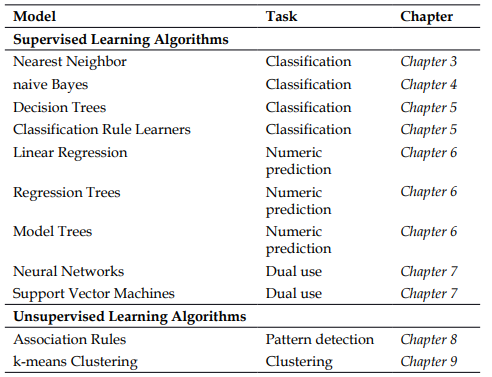
\includegraphics{Tipos de algoritmos.png}

}

\caption{Figura 1. Tipos de algoritmos}

\end{figure}

Para hacer doincidir una tarea de aprendizaje con un enfoque
autom{[}atico es necesario comenzar con 4 tipos de tareas:

\begin{itemize}
\item
  Clasificación
\item
  Predicción numérica
\item
  Detección de patrones
\item
  Agrupación
\end{itemize}

\hypertarget{uso-de-r-para-el-aprendizaje-automuxe1tico}{%
\paragraph{Uso de R para el aprendizaje
automático}\label{uso-de-r-para-el-aprendizaje-automuxe1tico}}

Es una herramienta muy util para el el aprendizaje automático y gracias
a que es un código abierto no hay cargo adicional por funcionalidad, una
comunidad de expertos que contribuyen al software.

\hypertarget{instalaciuxf3n-y-carga-de-paquetes-r}{%
\subsubsection{Instalación y carga de paquetes
R}\label{instalaciuxf3n-y-carga-de-paquetes-r}}

La forma más directa de instalar un paquete es con la función
install.packages( ).

\[>install.packages("RWeka")\]

R se conectará a CRAN y descargará el paquete en el formato correcto
para su sistema operativo.

Si necesita instalar un paquete desde otra ubicación se puede usar el
siguiente comando:

\[>install.packages("RWeka", lib="/path/to/library")\]

\hypertarget{gestiuxf3n-y-comprender-los-datos}{%
\section{Gestión y comprender los
datos}\label{gestiuxf3n-y-comprender-los-datos}}

\hypertarget{estructuras-de-datos-r}{%
\subsubsection{Estructuras de datos R}\label{estructuras-de-datos-r}}

Las estructuras de datos que se utilizan en R están diseñadas con el fin
de facilitar la manipulación de los datos, las estructuras más
utilizadas son: vectores, factores, listas, matrices y data frames.

\hypertarget{vectores}{%
\subsubsection{Vectores}\label{vectores}}

Estructura fundamental, almacena un conjunto ordenado de valores llamdo
elementos. Dentro del vector todos los elementos deben ser del mismo
tipo.

Existen varios tipos de vectores:

\begin{itemize}
\item
  Entero: sin decimales
\item
  Numérico: con decimales
\item
  Personajes: datos de texto
\item
  Lógico: Verdadero o falso
\end{itemize}

Para la creación de vectores se puede utilizar:

\begin{Shaded}
\begin{Highlighting}[]
\NormalTok{subject\_name }\OtherTok{\textless{}{-}} \FunctionTok{c}\NormalTok{(}\StringTok{"John Doe"}\NormalTok{, }\StringTok{"Jane Doe"}\NormalTok{, }\StringTok{"Steve Graves"}\NormalTok{)}
\NormalTok{temperature }\OtherTok{\textless{}{-}} \FunctionTok{c}\NormalTok{(}\FloatTok{98.1}\NormalTok{, }\FloatTok{98.6}\NormalTok{,}\FloatTok{101.4}\NormalTok{)}
\NormalTok{flu\_status }\OtherTok{\textless{}{-}} \FunctionTok{c}\NormalTok{(}\ConstantTok{FALSE}\NormalTok{, }\ConstantTok{FALSE}\NormalTok{, }\ConstantTok{TRUE}\NormalTok{)}
\end{Highlighting}
\end{Shaded}

Para lograr extraer un dato específico se utiliza el comando:

\begin{Shaded}
\begin{Highlighting}[]
\NormalTok{temperature[}\DecValTok{2}\NormalTok{]}
\end{Highlighting}
\end{Shaded}

\begin{verbatim}
[1] 98.6
\end{verbatim}

\begin{Shaded}
\begin{Highlighting}[]
\NormalTok{temperature[}\DecValTok{2}\SpecialCharTok{:}\DecValTok{3}\NormalTok{]}
\end{Highlighting}
\end{Shaded}

\begin{verbatim}
[1]  98.6 101.4
\end{verbatim}

Para excluir valores se puede utilizar el símbolo (-):

\begin{Shaded}
\begin{Highlighting}[]
\NormalTok{temperature[}\SpecialCharTok{{-}}\DecValTok{2}\NormalTok{]}
\end{Highlighting}
\end{Shaded}

\begin{verbatim}
[1]  98.1 101.4
\end{verbatim}

Otra forma para excluir datos es con el siguiente comando:

\begin{Shaded}
\begin{Highlighting}[]
\NormalTok{temperature[}\FunctionTok{c}\NormalTok{(}\ConstantTok{TRUE}\NormalTok{, }\ConstantTok{TRUE}\NormalTok{, }\ConstantTok{FALSE}\NormalTok{)]}
\end{Highlighting}
\end{Shaded}

\begin{verbatim}
[1] 98.1 98.6
\end{verbatim}

\hypertarget{factores}{%
\subsubsection{Factores}\label{factores}}

Los rasgos que representan una características con categorías de valores
son llamdos nominales.

Para este tipo de datos existe una estructura específica en R conocida
como factor, este es un caso especial de vector.

Para crear un factor a partir de un vector de character se debe aplicar
\emph{factor ( )}

\begin{Shaded}
\begin{Highlighting}[]
\NormalTok{gender }\OtherTok{\textless{}{-}} \FunctionTok{factor}\NormalTok{(}\FunctionTok{c}\NormalTok{(}\StringTok{"MALE"}\NormalTok{,}\StringTok{"FEMALE"}\NormalTok{, }\StringTok{"MALE"}\NormalTok{))}
\NormalTok{gender}
\end{Highlighting}
\end{Shaded}

\begin{verbatim}
[1] MALE   FEMALE MALE  
Levels: FEMALE MALE
\end{verbatim}

Los niveles comprenden un conjunto de posibles categor{[}ia que
podr{[}ian tomar los datos, al crear factores se puede agregar niveles
adicionales:

\begin{Shaded}
\begin{Highlighting}[]
\NormalTok{blood }\OtherTok{\textless{}{-}} \FunctionTok{factor}\NormalTok{(}\FunctionTok{c}\NormalTok{(}\StringTok{"O"}\NormalTok{,}\StringTok{"AB"}\NormalTok{,}\StringTok{"A"}\NormalTok{),}\AttributeTok{levels=}\FunctionTok{c}\NormalTok{(}\StringTok{"A"}\NormalTok{,}\StringTok{"B"}\NormalTok{,}\StringTok{"AB"}\NormalTok{,}\StringTok{"O"}\NormalTok{))}
\NormalTok{blood}
\end{Highlighting}
\end{Shaded}

\begin{verbatim}
[1] O  AB A 
Levels: A B AB O
\end{verbatim}

\hypertarget{listas}{%
\subsubsection{LISTAS}\label{listas}}

Se utiliza para almacenar un conjunto ordenado de valores. Permite
recopilar diferentes tipos de valores:

\begin{Shaded}
\begin{Highlighting}[]
\NormalTok{subject\_name[}\DecValTok{1}\NormalTok{]}
\end{Highlighting}
\end{Shaded}

\begin{verbatim}
[1] "John Doe"
\end{verbatim}

\begin{Shaded}
\begin{Highlighting}[]
\NormalTok{temperature[}\DecValTok{1}\NormalTok{]}
\end{Highlighting}
\end{Shaded}

\begin{verbatim}
[1] 98.1
\end{verbatim}

\begin{Shaded}
\begin{Highlighting}[]
\NormalTok{flu\_status[}\DecValTok{1}\NormalTok{]}
\end{Highlighting}
\end{Shaded}

\begin{verbatim}
[1] FALSE
\end{verbatim}

\begin{Shaded}
\begin{Highlighting}[]
\NormalTok{gender[}\DecValTok{1}\NormalTok{]}
\end{Highlighting}
\end{Shaded}

\begin{verbatim}
[1] MALE
Levels: FEMALE MALE
\end{verbatim}

\begin{Shaded}
\begin{Highlighting}[]
\NormalTok{blood[}\DecValTok{1}\NormalTok{]}
\end{Highlighting}
\end{Shaded}

\begin{verbatim}
[1] O
Levels: A B AB O
\end{verbatim}

Esta estructura no permite agregar todos los datos m{[}edicos de un
paciente en un objeto que se utilice de manera repetida. Similar al
comando anterior se utiliza el comando list( ), adem{[}as de permitir
asignar un nombre para cada valor en la secuencia.

\begin{Shaded}
\begin{Highlighting}[]
\NormalTok{subject1 }\OtherTok{\textless{}{-}} \FunctionTok{list}\NormalTok{(}\AttributeTok{fullname =}\NormalTok{ subject\_name[}\DecValTok{1}\NormalTok{],}
\AttributeTok{temperature =}\NormalTok{ temperature[}\DecValTok{1}\NormalTok{],}
\AttributeTok{flu\_status =}\NormalTok{ flu\_status[}\DecValTok{1}\NormalTok{],}
\AttributeTok{gender =}\NormalTok{ gender[}\DecValTok{1}\NormalTok{],}
\AttributeTok{blood =}\NormalTok{ blood[}\DecValTok{1}\NormalTok{])}
\end{Highlighting}
\end{Shaded}

Para poder visualizar los datos se utiliza:

\begin{Shaded}
\begin{Highlighting}[]
\NormalTok{subject1}\SpecialCharTok{$}\NormalTok{fullname}
\end{Highlighting}
\end{Shaded}

\begin{verbatim}
[1] "John Doe"
\end{verbatim}

\begin{Shaded}
\begin{Highlighting}[]
\NormalTok{subject1}\SpecialCharTok{$}\NormalTok{temperature}
\end{Highlighting}
\end{Shaded}

\begin{verbatim}
[1] 98.1
\end{verbatim}

\begin{Shaded}
\begin{Highlighting}[]
\NormalTok{subject1}\SpecialCharTok{$}\NormalTok{flu\_status}
\end{Highlighting}
\end{Shaded}

\begin{verbatim}
[1] FALSE
\end{verbatim}

\begin{Shaded}
\begin{Highlighting}[]
\NormalTok{subject1}\SpecialCharTok{$}\NormalTok{gender}
\end{Highlighting}
\end{Shaded}

\begin{verbatim}
[1] MALE
Levels: FEMALE MALE
\end{verbatim}

\begin{Shaded}
\begin{Highlighting}[]
\NormalTok{subject1}\SpecialCharTok{$}\NormalTok{blood}
\end{Highlighting}
\end{Shaded}

\begin{verbatim}
[1] O
Levels: A B AB O
\end{verbatim}

\begin{Shaded}
\begin{Highlighting}[]
\NormalTok{subject1[}\DecValTok{2}\NormalTok{]}
\end{Highlighting}
\end{Shaded}

\begin{verbatim}
$temperature
[1] 98.1
\end{verbatim}

\begin{Shaded}
\begin{Highlighting}[]
\NormalTok{subject1}\SpecialCharTok{$}\NormalTok{temperatura}
\end{Highlighting}
\end{Shaded}

\begin{verbatim}
NULL
\end{verbatim}

\begin{Shaded}
\begin{Highlighting}[]
\NormalTok{subject1[}\FunctionTok{c}\NormalTok{(}\StringTok{"temperatura"}\NormalTok{, }\StringTok{"estado\_gripe"}\NormalTok{)]}\SpecialCharTok{$}\NormalTok{temperatura}
\end{Highlighting}
\end{Shaded}

\begin{verbatim}
NULL
\end{verbatim}

\begin{Shaded}
\begin{Highlighting}[]
\NormalTok{subject1[}\FunctionTok{c}\NormalTok{(}\StringTok{"temperatura"}\NormalTok{, }\StringTok{"estado\_gripe"}\NormalTok{)]}\SpecialCharTok{$}\NormalTok{estado\_gripe}
\end{Highlighting}
\end{Shaded}

\begin{verbatim}
NULL
\end{verbatim}

\hypertarget{data-frames}{%
\subsubsection{Data frames}\label{data-frames}}

La estructura de datos de R más importante utilizada en el aprendizaje
automático es data frames, esta estructura es similar a una hoja de
cálculo (filas, columnas). Para explicar como crear un data frame
utilizaremos los vectores de datos de pacientes que anteriormente se
crearon.

\begin{Shaded}
\begin{Highlighting}[]
\NormalTok{pt\_data }\OtherTok{\textless{}{-}} \FunctionTok{data.frame}\NormalTok{(subject\_name, temperature, flu\_status,gender, blood, }\AttributeTok{stringsAsFactors =} \ConstantTok{FALSE}\NormalTok{)}
\end{Highlighting}
\end{Shaded}

Como se observa se adiciono el parámetro stringsAsFactors = FALSE, al
especificar esta opción impedimos que R convierta cada vector de
caracteres en un factor. Los datos se muestran en forma de matriz.

\begin{Shaded}
\begin{Highlighting}[]
\NormalTok{pt\_data}
\end{Highlighting}
\end{Shaded}

\begin{verbatim}
  subject_name temperature flu_status gender blood
1     John Doe        98.1      FALSE   MALE     O
2     Jane Doe        98.6      FALSE FEMALE    AB
3 Steve Graves       101.4       TRUE   MALE     A
\end{verbatim}

Para extraer columnas enteras la forma más directa es referirse por el
nombre:

\begin{Shaded}
\begin{Highlighting}[]
\NormalTok{ pt\_data}\SpecialCharTok{$}\NormalTok{subject\_name}
\end{Highlighting}
\end{Shaded}

\begin{verbatim}
[1] "John Doe"     "Jane Doe"     "Steve Graves"
\end{verbatim}

\begin{Shaded}
\begin{Highlighting}[]
\NormalTok{ pt\_data[}\FunctionTok{c}\NormalTok{(}\StringTok{"temperature"}\NormalTok{, }\StringTok{"flu\_status"}\NormalTok{)]}
\end{Highlighting}
\end{Shaded}

\begin{verbatim}
  temperature flu_status
1        98.1      FALSE
2        98.6      FALSE
3       101.4       TRUE
\end{verbatim}

Podemos extraer valores del data frame, sin embargo se debe especificar
la posición de las filas (primero) y columnas (segundo).

\begin{Shaded}
\begin{Highlighting}[]
\NormalTok{pt\_data[}\DecValTok{1}\NormalTok{, }\DecValTok{2}\NormalTok{]}
\end{Highlighting}
\end{Shaded}

\begin{verbatim}
[1] 98.1
\end{verbatim}

En caso de necesitar mas de una fila o columna se lo debe escribir de la
siguiente manera:

\begin{Shaded}
\begin{Highlighting}[]
\NormalTok{ pt\_data[}\FunctionTok{c}\NormalTok{(}\DecValTok{1}\NormalTok{, }\DecValTok{3}\NormalTok{), }\FunctionTok{c}\NormalTok{(}\DecValTok{2}\NormalTok{, }\DecValTok{4}\NormalTok{)]}
\end{Highlighting}
\end{Shaded}

\begin{verbatim}
  temperature gender
1        98.1   MALE
3       101.4   MALE
\end{verbatim}

Para extraer todas las filas o columnas, se debe dejar en blanco la
parte de la fila o columna.

\begin{Shaded}
\begin{Highlighting}[]
\NormalTok{pt\_data[, }\DecValTok{1}\NormalTok{]}
\end{Highlighting}
\end{Shaded}

\begin{verbatim}
[1] "John Doe"     "Jane Doe"     "Steve Graves"
\end{verbatim}

\begin{Shaded}
\begin{Highlighting}[]
\NormalTok{pt\_data[}\DecValTok{1}\NormalTok{, ]}
\end{Highlighting}
\end{Shaded}

\begin{verbatim}
  subject_name temperature flu_status gender blood
1     John Doe        98.1      FALSE   MALE     O
\end{verbatim}

\begin{Shaded}
\begin{Highlighting}[]
\NormalTok{pt\_data[ , ]}
\end{Highlighting}
\end{Shaded}

\begin{verbatim}
  subject_name temperature flu_status gender blood
1     John Doe        98.1      FALSE   MALE     O
2     Jane Doe        98.6      FALSE FEMALE    AB
3 Steve Graves       101.4       TRUE   MALE     A
\end{verbatim}

Asi mismo para extraer valores en lista o excluir valores se puede
utilizar los comandos que se utilizaron en vectores y listas.

\begin{Shaded}
\begin{Highlighting}[]
\NormalTok{pt\_data[}\FunctionTok{c}\NormalTok{(}\DecValTok{1}\NormalTok{, }\DecValTok{3}\NormalTok{), }\FunctionTok{c}\NormalTok{(}\StringTok{"temperature"}\NormalTok{, }\StringTok{"gender"}\NormalTok{)]}
\end{Highlighting}
\end{Shaded}

\begin{verbatim}
  temperature gender
1        98.1   MALE
3       101.4   MALE
\end{verbatim}

\begin{Shaded}
\begin{Highlighting}[]
\NormalTok{pt\_data[}\SpecialCharTok{{-}}\DecValTok{2}\NormalTok{, }\FunctionTok{c}\NormalTok{(}\SpecialCharTok{{-}}\DecValTok{1}\NormalTok{, }\SpecialCharTok{{-}}\DecValTok{3}\NormalTok{, }\SpecialCharTok{{-}}\DecValTok{5}\NormalTok{)]}
\end{Highlighting}
\end{Shaded}

\begin{verbatim}
  temperature gender
1        98.1   MALE
3       101.4   MALE
\end{verbatim}

\hypertarget{matrices-y-arrays}{%
\subsubsection{MATRICES Y ARRAYS}\label{matrices-y-arrays}}

La matriz es una estructura bidimensional que puede contener cualquier
tipo de de datos, aunque por lo general almacena datos numericos debido
a que es utilizada para operaciones matemáticas.

Para crear una matriz se utiliza la función matrix( ) :

\begin{Shaded}
\begin{Highlighting}[]
\NormalTok{m }\OtherTok{\textless{}{-}} \FunctionTok{matrix}\NormalTok{(}\FunctionTok{c}\NormalTok{(}\StringTok{\textquotesingle{}a\textquotesingle{}}\NormalTok{, }\StringTok{\textquotesingle{}b\textquotesingle{}}\NormalTok{, }\StringTok{\textquotesingle{}c\textquotesingle{}}\NormalTok{, }\StringTok{\textquotesingle{}d\textquotesingle{}}\NormalTok{), }\AttributeTok{nrow =} \DecValTok{2}\NormalTok{)}
\NormalTok{m}
\end{Highlighting}
\end{Shaded}

\begin{verbatim}
     [,1] [,2]
[1,] "a"  "c" 
[2,] "b"  "d" 
\end{verbatim}

\begin{Shaded}
\begin{Highlighting}[]
\NormalTok{m1 }\OtherTok{\textless{}{-}} \FunctionTok{matrix}\NormalTok{(}\FunctionTok{c}\NormalTok{(}\StringTok{\textquotesingle{}a\textquotesingle{}}\NormalTok{, }\StringTok{\textquotesingle{}b\textquotesingle{}}\NormalTok{, }\StringTok{\textquotesingle{}c\textquotesingle{}}\NormalTok{, }\StringTok{\textquotesingle{}d\textquotesingle{}}\NormalTok{), }\AttributeTok{ncol =} \DecValTok{2}\NormalTok{)}
\NormalTok{m1}
\end{Highlighting}
\end{Shaded}

\begin{verbatim}
     [,1] [,2]
[1,] "a"  "c" 
[2,] "b"  "d" 
\end{verbatim}

Con este comando R carga primero la columna 1 de la matriz y luego la
columna 2, esto se le conoce como orden de columna principal. Veamos un
ejemplo con 6 valores:

\begin{Shaded}
\begin{Highlighting}[]
\NormalTok{m }\OtherTok{\textless{}{-}} \FunctionTok{matrix}\NormalTok{(}\FunctionTok{c}\NormalTok{(}\StringTok{\textquotesingle{}a\textquotesingle{}}\NormalTok{, }\StringTok{\textquotesingle{}b\textquotesingle{}}\NormalTok{, }\StringTok{\textquotesingle{}c\textquotesingle{}}\NormalTok{, }\StringTok{\textquotesingle{}d\textquotesingle{}}\NormalTok{, }\StringTok{\textquotesingle{}e\textquotesingle{}}\NormalTok{, }\StringTok{\textquotesingle{}f\textquotesingle{}}\NormalTok{), }\AttributeTok{nrow =} \DecValTok{2}\NormalTok{)}
\NormalTok{m}
\end{Highlighting}
\end{Shaded}

\begin{verbatim}
     [,1] [,2] [,3]
[1,] "a"  "c"  "e" 
[2,] "b"  "d"  "f" 
\end{verbatim}

\begin{Shaded}
\begin{Highlighting}[]
\NormalTok{m1 }\OtherTok{\textless{}{-}} \FunctionTok{matrix}\NormalTok{(}\FunctionTok{c}\NormalTok{(}\StringTok{\textquotesingle{}a\textquotesingle{}}\NormalTok{, }\StringTok{\textquotesingle{}b\textquotesingle{}}\NormalTok{, }\StringTok{\textquotesingle{}c\textquotesingle{}}\NormalTok{, }\StringTok{\textquotesingle{}d\textquotesingle{}}\NormalTok{, }\StringTok{\textquotesingle{}e\textquotesingle{}}\NormalTok{, }\StringTok{\textquotesingle{}f\textquotesingle{}}\NormalTok{), }\AttributeTok{ncol =} \DecValTok{2}\NormalTok{)}
\NormalTok{m1}
\end{Highlighting}
\end{Shaded}

\begin{verbatim}
     [,1] [,2]
[1,] "a"  "d" 
[2,] "b"  "e" 
[3,] "c"  "f" 
\end{verbatim}

Al igual que los data frame los valores de las matrices se puede extraer
usando {[}fila, columna{]}

\begin{Shaded}
\begin{Highlighting}[]
\NormalTok{ m[}\DecValTok{1}\NormalTok{, ]}
\end{Highlighting}
\end{Shaded}

\begin{verbatim}
[1] "a" "c" "e"
\end{verbatim}

\begin{Shaded}
\begin{Highlighting}[]
\NormalTok{ m[, }\DecValTok{1}\NormalTok{]}
\end{Highlighting}
\end{Shaded}

\begin{verbatim}
[1] "a" "b"
\end{verbatim}

\hypertarget{gestion-de-datos-con-r}{%
\subsubsection{GESTION DE DATOS CON R}\label{gestion-de-datos-con-r}}

Las herramientas de R para cargar datos son muy utiles a la hora de
trabajar con conjuntos de datos extensos.

\hypertarget{guardar-y-cargar-estructuras-de-datos-r}{%
\paragraph{GUARDAR Y CARGAR ESTRUCTURAS DE DATOS
R}\label{guardar-y-cargar-estructuras-de-datos-r}}

Para una estructura de datos en particular en un archivo que pueda
volver a cargarse más tarde, puede usar la funcion save( ) la cual
permite estructuras de datos R en la ubicacion deseada. Se puede guardar
los archivos en una extension RData.

\begin{Shaded}
\begin{Highlighting}[]
\CommentTok{\#save(x, y, z, file = "mydata.RData")}
\end{Highlighting}
\end{Shaded}

El comando load( ) recreará las estructuras de datos ya guardadas que se
encuentran en RData.

\begin{Shaded}
\begin{Highlighting}[]
\CommentTok{\#load("mydata.RData")}
\end{Highlighting}
\end{Shaded}

\hypertarget{importar-y-guardar-datos-de-archivos-csv}{%
\subsubsection{IMPORTAR Y GUARDAR DATOS DE ARCHIVOS
CSV}\label{importar-y-guardar-datos-de-archivos-csv}}

Existen varios formatos para almacenar los datos publicamente, los
archivos de texto son un claro ejemplo de esto y es considerado casi
universal.

Un archivo de datos tabular tiene una estructura de matriz, de modo que
se pueda tener en cada fila un ejemplo y el mismo número de
características, los valores de estas características se encuentran
separadas por un delimitador (símbolo predefinido) .

El archivo de datos tabular más conocido es el Comma Separated Values
(CSV) el cual utiliza una coma como delimitador, estos pueden importarse
o exportarse desde varias aplicaciones comunes.

Para cargar este archivo se utiliza:

\begin{Shaded}
\begin{Highlighting}[]
\CommentTok{\#pt\_data \textless{}{-} read.csv("pt\_data.csv", stringsAsFactors = FALSE)}
\end{Highlighting}
\end{Shaded}

Si sus datos no se encuentran en el directorio se puede especificar la
ruta del archivo CSV. Al llamar la funcion read.csv( ) por defecto R
asume que el archivo incluye un encabezado con los nombres de las
características del conjunto de datos, en caso de no tenerlo se debe
especificar con la opción header=FALSE.

\begin{Shaded}
\begin{Highlighting}[]
\CommentTok{\#mydata \textless{}{-} read.csv("mydata.csv", stringsAsFactors = FALSE,header = FALSE)}
\end{Highlighting}
\end{Shaded}

Para guardar un data frame en un archivo CSV se utiliza la opción write:

\begin{Shaded}
\begin{Highlighting}[]
\CommentTok{\#write.csv(pt\_data, file = "pt\_data.csv")}
\end{Highlighting}
\end{Shaded}

\hypertarget{importacion-de-datos-de-bases-de-datos-sql}{%
\subsubsection{IMPORTACION DE DATOS DE BASES DE DATOS
SQL}\label{importacion-de-datos-de-bases-de-datos-sql}}

Se necesita instalar RODBC:

\begin{Shaded}
\begin{Highlighting}[]
\CommentTok{\#install.packages("RODBC")}
\CommentTok{\#library(RODBC)}
\end{Highlighting}
\end{Shaded}

Se abre la conexión llamada mydb la base de datos con el DSNmi\_dsn:

\begin{Shaded}
\begin{Highlighting}[]
\CommentTok{\#mydb \textless{}{-} odbcConnect("my\_dsn")}
\end{Highlighting}
\end{Shaded}

SI su conexión requiere de un nombre de usuario y una contraseña se debe
especificar al llamar la funcion odbcConnect( ):

\begin{Shaded}
\begin{Highlighting}[]
\CommentTok{\#mydb \textless{}{-} odbcConnect("my\_dsn", uid = "my\_username", pwd = "my\_password")}
\end{Highlighting}
\end{Shaded}

La función sqlQuery( ) utiliza consultas SQL típicas como se muestra:

\begin{Shaded}
\begin{Highlighting}[]
\CommentTok{\#patient\_query \textless{}{-} "select * from patient\_data where alive = 1"}
\CommentTok{\#patient\_data \textless{}{-} sqlQuery(channel = mydb, query = patient\_query, \#stringsAsFactors = FALSE)}
\end{Highlighting}
\end{Shaded}

Se cierra la conexión con:

\begin{Shaded}
\begin{Highlighting}[]
\CommentTok{\#odbcClose(mydb)}
\end{Highlighting}
\end{Shaded}

\hypertarget{exploraciuxf3n-y-comprensiuxf3n-de-datos}{%
\subsubsection{EXPLORACIÓN Y COMPRENSIÓN DE
DATOS}\label{exploraciuxf3n-y-comprensiuxf3n-de-datos}}

El siguiente paso en el proceso de aprensizaje automático es examinar
los datos, para esto cargaremos los datos utilizando el read.csv( ).

\begin{Shaded}
\begin{Highlighting}[]
\NormalTok{usedcars }\OtherTok{\textless{}{-}} \FunctionTok{read.csv}\NormalTok{(}\StringTok{"usedcars.csv"}\NormalTok{, }\AttributeTok{stringsAsFactors =} \ConstantTok{FALSE}\NormalTok{)}
\end{Highlighting}
\end{Shaded}

\hypertarget{exploranco-la-estructura-de-los-datos}{%
\paragraph{Exploranco la estructura de los
datos}\label{exploranco-la-estructura-de-los-datos}}

Para esto usar la función str( ) proporciona un método para mostrar el
data frame o cualquier estructura, se utiliza para crear el esquema
básico de nuestro data dictionary:

\begin{Shaded}
\begin{Highlighting}[]
\FunctionTok{str}\NormalTok{(usedcars)}
\end{Highlighting}
\end{Shaded}

\begin{verbatim}
'data.frame':   150 obs. of  6 variables:
 $ year        : int  2011 2011 2011 2011 2012 2010 2011 2010 2011 2010 ...
 $ model       : chr  "SEL" "SEL" "SEL" "SEL" ...
 $ price       : int  21992 20995 19995 17809 17500 17495 17000 16995 16995 16995 ...
 $ mileage     : int  7413 10926 7351 11613 8367 25125 27393 21026 32655 36116 ...
 $ color       : chr  "Yellow" "Gray" "Silver" "Gray" ...
 $ transmission: chr  "AUTO" "AUTO" "AUTO" "AUTO" ...
\end{verbatim}

Se puede extraer las características de los datos como la característica
color:

\begin{Shaded}
\begin{Highlighting}[]
\NormalTok{usedcars}\SpecialCharTok{$}\NormalTok{color}
\end{Highlighting}
\end{Shaded}

\begin{verbatim}
  [1] "Yellow" "Gray"   "Silver" "Gray"   "White"  "Silver" "Blue"   "Silver"
  [9] "Silver" "Silver" "Black"  "Silver" "Green"  "Red"    "White"  "Blue"  
 [17] "Silver" "Silver" "Blue"   "Silver" "Silver" "White"  "Silver" "Black" 
 [25] "Blue"   "Blue"   "Black"  "Black"  "Gray"   "Silver" "Red"    "Black" 
 [33] "Black"  "Black"  "Red"    "Black"  "White"  "Silver" "White"  "White" 
 [41] "Black"  "Gray"   "Black"  "Silver" "Red"    "Silver" "Black"  "Blue"  
 [49] "Gray"   "Red"    "Black"  "Black"  "Silver" "Red"    "Black"  "Silver"
 [57] "Black"  "Black"  "Silver" "Silver" "Green"  "Gray"   "Black"  "Silver"
 [65] "Black"  "Black"  "Blue"   "Gray"   "White"  "Blue"   "Black"  "Black" 
 [73] "Gray"   "Silver" "Red"    "Red"    "Black"  "Gray"   "Black"  "Blue"  
 [81] "Blue"   "Blue"   "Red"    "Black"  "Black"  "White"  "Blue"   "Red"   
 [89] "Gray"   "Red"    "Gray"   "Silver" "Gray"   "Silver" "Black"  "Black" 
 [97] "Blue"   "Blue"   "Gray"   "White"  "White"  "Red"    "Blue"   "Black" 
[105] "Black"  "Red"    "Green"  "Black"  "Red"    "Silver" "Red"    "Red"   
[113] "Blue"   "Gray"   "Red"    "Gray"   "Gold"   "Green"  "Red"    "Silver"
[121] "Black"  "Red"    "Silver" "Black"  "Silver" "White"  "White"  "Blue"  
[129] "Red"    "Silver" "Silver" "White"  "Black"  "Silver" "White"  "Yellow"
[137] "Black"  "Red"    "White"  "Red"    "Silver" "White"  "Green"  "Gray"  
[145] "Black"  "Silver" "Red"    "Red"    "Yellow" "Red"   
\end{verbatim}

\hypertarget{explorando-variables-numuxe9ricas}{%
\paragraph{Explorando variables
numéricas}\label{explorando-variables-numuxe9ricas}}

Para conocer las variables numéricas se emplea un conjunto de medidas de
uso común llamado summary statistics (resumen estadístico), esta función
muestra estadísticas comunes resumidas:

\begin{Shaded}
\begin{Highlighting}[]
\FunctionTok{summary}\NormalTok{(usedcars}\SpecialCharTok{$}\NormalTok{year)}
\end{Highlighting}
\end{Shaded}

\begin{verbatim}
   Min. 1st Qu.  Median    Mean 3rd Qu.    Max. 
   2000    2008    2009    2009    2010    2012 
\end{verbatim}

este función también se la puede usar para obtener estadísticas de
varias variables numéricas al mismo tiempo:

\begin{Shaded}
\begin{Highlighting}[]
\FunctionTok{summary}\NormalTok{(usedcars[}\FunctionTok{c}\NormalTok{(}\StringTok{"price"}\NormalTok{, }\StringTok{"mileage"}\NormalTok{)])}
\end{Highlighting}
\end{Shaded}

\begin{verbatim}
     price          mileage      
 Min.   : 3800   Min.   :  4867  
 1st Qu.:10995   1st Qu.: 27200  
 Median :13592   Median : 36385  
 Mean   :12962   Mean   : 44261  
 3rd Qu.:14904   3rd Qu.: 55125  
 Max.   :21992   Max.   :151479  
\end{verbatim}

\hypertarget{mediciuxf3n-de-la-tendencia-central-media-y-mediana}{%
\paragraph{Medición de la tendencia central: media y
mediana}\label{mediciuxf3n-de-la-tendencia-central-media-y-mediana}}

El promedio es una medida definida como la suma de todos los valores
dividida para el número de valores.

\begin{Shaded}
\begin{Highlighting}[]
\NormalTok{(}\DecValTok{36000} \SpecialCharTok{+} \DecValTok{44000} \SpecialCharTok{+} \DecValTok{56000}\NormalTok{) }\SpecialCharTok{/} \DecValTok{3}
\end{Highlighting}
\end{Shaded}

\begin{verbatim}
[1] 45333.33
\end{verbatim}

Existe una función dentro de R para realizar esta operación:

\begin{Shaded}
\begin{Highlighting}[]
\FunctionTok{mean}\NormalTok{(}\FunctionTok{c}\NormalTok{(}\DecValTok{36000}\NormalTok{, }\DecValTok{44000}\NormalTok{, }\DecValTok{56000}\NormalTok{))}
\end{Highlighting}
\end{Shaded}

\begin{verbatim}
[1] 45333.33
\end{verbatim}

Por otro lado la mediana es una medida de tendencia central que
representa el valor de la mitad de una lista ordenada de valores. Para
esto utilizaremos la fórmula de R:

\begin{Shaded}
\begin{Highlighting}[]
\FunctionTok{median}\NormalTok{(}\FunctionTok{c}\NormalTok{(}\DecValTok{36000}\NormalTok{, }\DecValTok{44000}\NormalTok{, }\DecValTok{56000}\NormalTok{))}
\end{Highlighting}
\end{Shaded}

\begin{verbatim}
[1] 44000
\end{verbatim}

\hypertarget{mediciuxf3n-de-la-dispersiuxf3n-cuartiles-y-resumen-de-cinco-nuxfameros}{%
\paragraph{Medición de la dispersión: Cuartiles y resumen de cinco
números}\label{mediciuxf3n-de-la-dispersiuxf3n-cuartiles-y-resumen-de-cinco-nuxfameros}}

Para poder conocer la diversidad de los datos es necesario utilizar
otras estadísticas resumidas, en este caso el resumen de cinco números.

Resumen de cinco numeros: conjunto de 5 estadíticas que representan una
aproximación de la dispersión de datos:

\begin{itemize}
\item
  Mínimo (mín)
\item
  Primer cuartil (Q1)
\item
  Mediana (Q2)
\item
  Tercer cuartil (Q3)
\item
  Máximo (máx)
\item
  Rango: Diferencia entre el valor mínimo y máximo. Dentro de R se
  utilizan 2 funciones range( ) y diff( ) para calcular el rango con un
  solo comando.

\begin{Shaded}
\begin{Highlighting}[]
\FunctionTok{range}\NormalTok{(usedcars}\SpecialCharTok{$}\NormalTok{price)}
\end{Highlighting}
\end{Shaded}

\begin{verbatim}
[1]  3800 21992
\end{verbatim}

\begin{Shaded}
\begin{Highlighting}[]
\FunctionTok{diff}\NormalTok{(}\FunctionTok{range}\NormalTok{(usedcars}\SpecialCharTok{$}\NormalTok{price))}
\end{Highlighting}
\end{Shaded}

\begin{verbatim}
[1] 18192
\end{verbatim}
\end{itemize}

Q1 y Q3 son el valor por debajo o por encima del cual se encuentra una
cuarta parte de los valores, su diferencia se conoce como rango
intercuartil (IQR):

\begin{Shaded}
\begin{Highlighting}[]
\FunctionTok{IQR}\NormalTok{(usedcars}\SpecialCharTok{$}\NormalTok{price)}
\end{Highlighting}
\end{Shaded}

\begin{verbatim}
[1] 3909.5
\end{verbatim}

La funcion cuantil devuelve el resumen de cinco números:

\begin{Shaded}
\begin{Highlighting}[]
\FunctionTok{quantile}\NormalTok{(usedcars}\SpecialCharTok{$}\NormalTok{price)}
\end{Highlighting}
\end{Shaded}

\begin{verbatim}
     0%     25%     50%     75%    100% 
 3800.0 10995.0 13591.5 14904.5 21992.0 
\end{verbatim}

Si se especifica el parámetro adicional probs mediante un vector que
denote puntos de corte se pued obtener cuantiles arbitrarios con
percentiles de 1 y 99:

\begin{Shaded}
\begin{Highlighting}[]
 \FunctionTok{quantile}\NormalTok{(usedcars}\SpecialCharTok{$}\NormalTok{price, }\AttributeTok{probs =} \FunctionTok{c}\NormalTok{(}\FloatTok{0.01}\NormalTok{, }\FloatTok{0.99}\NormalTok{))}
\end{Highlighting}
\end{Shaded}

\begin{verbatim}
      1%      99% 
 5428.69 20505.00 
\end{verbatim}

La función seq( ) se utiliza para generar vectores de valore sque esten
espaciados de manera uniforme:

\begin{Shaded}
\begin{Highlighting}[]
\FunctionTok{quantile}\NormalTok{(usedcars}\SpecialCharTok{$}\NormalTok{price, }\FunctionTok{seq}\NormalTok{(}\AttributeTok{from =} \DecValTok{0}\NormalTok{, }\AttributeTok{to =} \DecValTok{1}\NormalTok{, }\AttributeTok{by =} \FloatTok{0.20}\NormalTok{))}
\end{Highlighting}
\end{Shaded}

\begin{verbatim}
     0%     20%     40%     60%     80%    100% 
 3800.0 10759.4 12993.8 13992.0 14999.0 21992.0 
\end{verbatim}

\hypertarget{visualizaciuxf3n-de-varibales-numuxe9ricas-diagramas-de-caja}{%
\paragraph{Visualización de varibales numéricas: diagramas de
caja}\label{visualizaciuxf3n-de-varibales-numuxe9ricas-diagramas-de-caja}}

Una visualización común del resumen de cinco números es un diagrama de
caja, este grafico muestra el centro y la dispersión de una variable
numérica de modo que permite obtener una idea del rango y sesgo o para
la comparación con otras variables.

Al usar la funcion boxplot( ) se debe especificar algunos parámetros
adicionales, se utiliza el código de:

\begin{Shaded}
\begin{Highlighting}[]
\FunctionTok{boxplot}\NormalTok{(usedcars}\SpecialCharTok{$}\NormalTok{price, }\AttributeTok{main=}\StringTok{"Boxplot of Used Car Prices"}\NormalTok{, }\AttributeTok{ylab=}\StringTok{"Price ($)"}\NormalTok{)}
\end{Highlighting}
\end{Shaded}

\begin{figure}[H]

{\centering 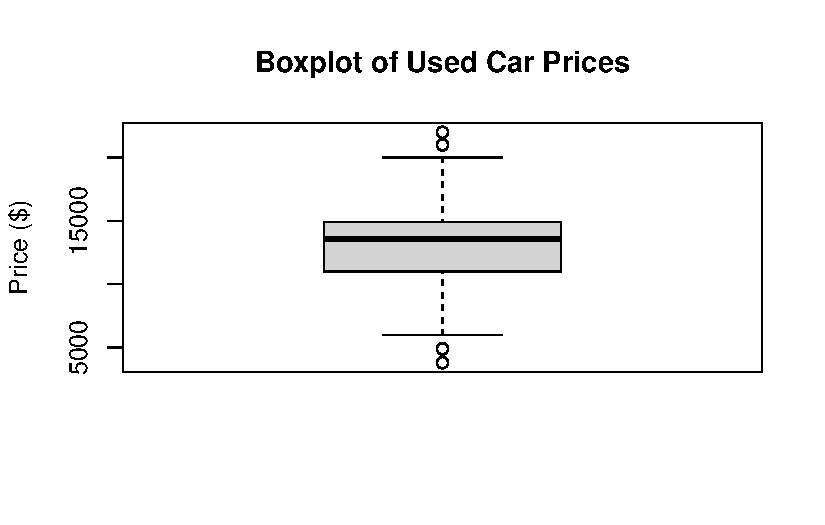
\includegraphics{Unidad1-resumen_files/figure-pdf/unnamed-chunk-54-1.pdf}

}

\end{figure}

\begin{Shaded}
\begin{Highlighting}[]
\FunctionTok{boxplot}\NormalTok{(usedcars}\SpecialCharTok{$}\NormalTok{mileage, }\AttributeTok{main=}\StringTok{"Boxplot of Used Car Mileage"}\NormalTok{, }\AttributeTok{ylab=}\StringTok{"Odometer (mi.)"}\NormalTok{)}
\end{Highlighting}
\end{Shaded}

\begin{figure}[H]

{\centering 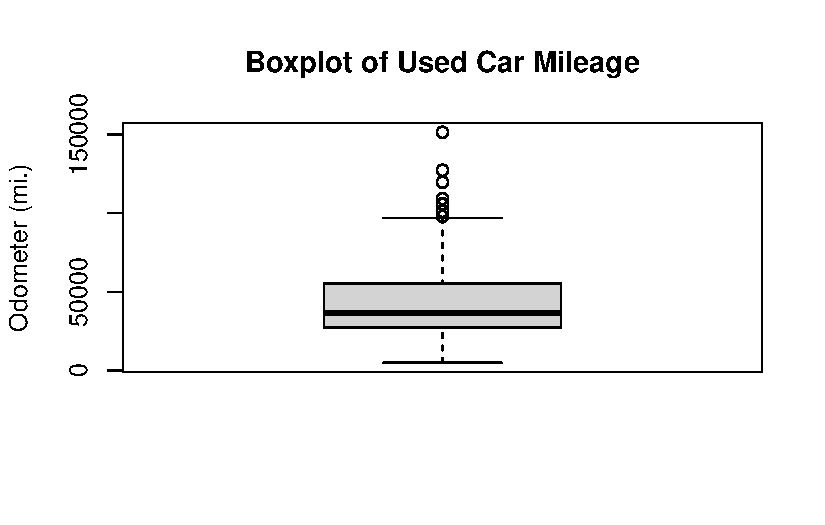
\includegraphics{Unidad1-resumen_files/figure-pdf/unnamed-chunk-54-2.pdf}

}

\end{figure}

Se muestran diagramas como se observan en la figura 2:

\begin{figure}

{\centering 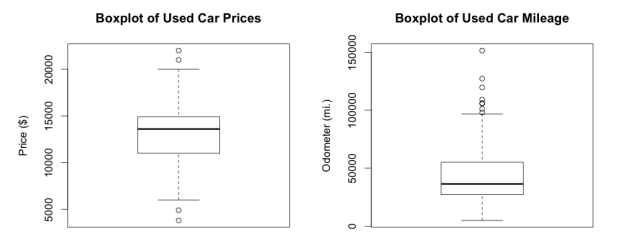
\includegraphics{Diagramas de caja.png}

}

\caption{Diagramas de caja}

\end{figure}

\hypertarget{visualizaciuxf3n-de-variables-numuxe9ricas---histogramas}{%
\paragraph{Visualización de variables numéricas -
histogramas}\label{visualizaciuxf3n-de-variables-numuxe9ricas---histogramas}}

Es histograma es una forma de representar graficamente la dispersión de
una variable numérica es similar a un diagrama de caja, divide los
valores de la variable en un número predefinido de porciones.

Se puede crear un histograma usando la función hist( ), al igual que en
el diagrama de caja se debe especificar un título para la figura.

\begin{Shaded}
\begin{Highlighting}[]
\FunctionTok{hist}\NormalTok{(usedcars}\SpecialCharTok{$}\NormalTok{price, }\AttributeTok{main =} \StringTok{"Histogram of Used Car Prices"}\NormalTok{, }\AttributeTok{xlab =} \StringTok{"Price ($)"}\NormalTok{)}
\end{Highlighting}
\end{Shaded}

\begin{figure}[H]

{\centering 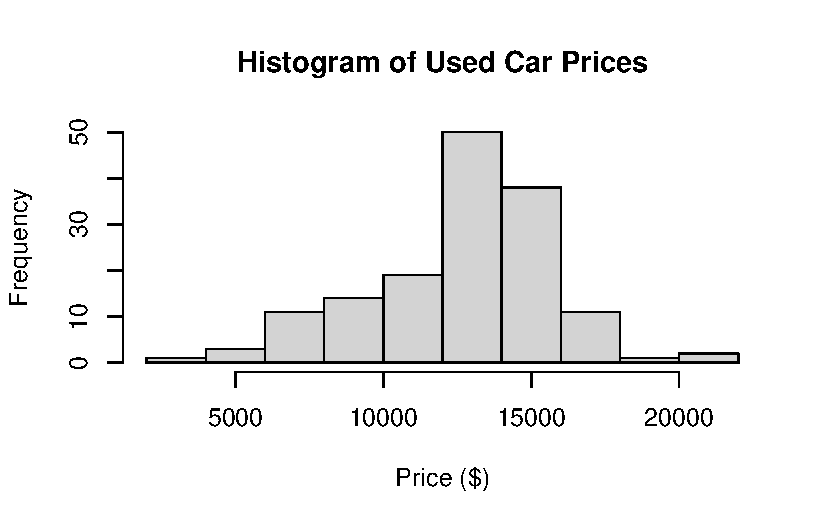
\includegraphics{Unidad1-resumen_files/figure-pdf/unnamed-chunk-55-1.pdf}

}

\end{figure}

\begin{Shaded}
\begin{Highlighting}[]
\FunctionTok{hist}\NormalTok{(usedcars}\SpecialCharTok{$}\NormalTok{mileage, }\AttributeTok{main =} \StringTok{"Histogram of Used Car Mileage"}\NormalTok{, }\AttributeTok{xlab =} \StringTok{"Odometer (mi.)"}\NormalTok{)}
\end{Highlighting}
\end{Shaded}

\begin{figure}[H]

{\centering 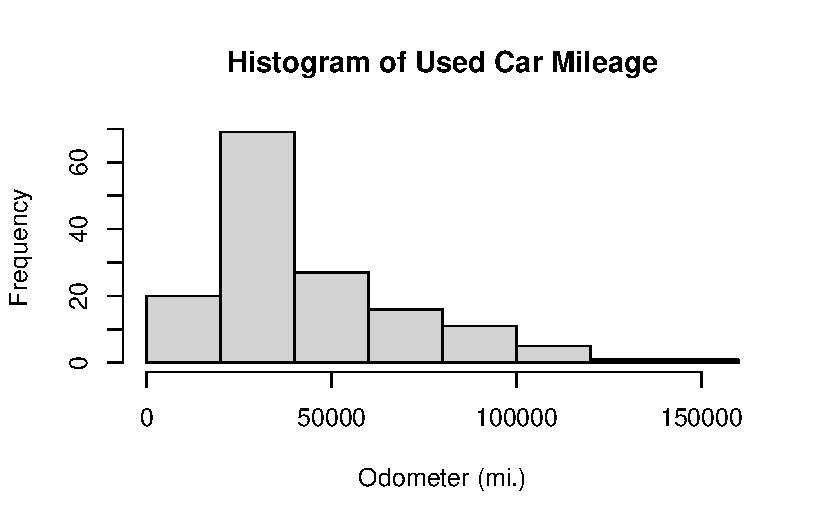
\includegraphics{Unidad1-resumen_files/figure-pdf/unnamed-chunk-55-2.pdf}

}

\end{figure}

\hypertarget{comprensiuxf3n-de-datos-numuxe9ricos-distribuciones-uniformes-y-normales}{%
\paragraph{Comprensión de datos numéricos: distribuciones uniformes y
normales}\label{comprensiuxf3n-de-datos-numuxe9ricos-distribuciones-uniformes-y-normales}}

La distribución de una variable describe la probabilidad de que un valor
caiga dentro de varios rangos, si todos los valores tienen la misma
probabilidad de ocurrir se dice que la distribución es uniforme, al
visualizarse en un histograma se lo puede observar de la siguiente
forma:

\begin{figure}

{\centering 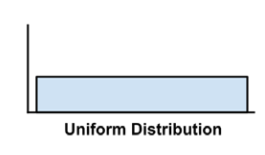
\includegraphics{distribucion uniforme.png}

}

\caption{Distribución uniforme}

\end{figure}

La distribución normal sucede cuando los valores tienen diferente
probabilidad de suceder, si lo visualizamos en un histograma se puede
observar una forma de campana.

\begin{figure}

{\centering 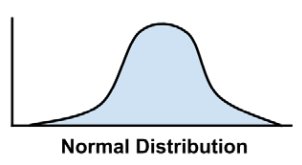
\includegraphics{normal.png}

}

\caption{Distribución normal}

\end{figure}

\hypertarget{mediciuxf3n-de-la-dispersiuxf3n-varianza-y-desviaciuxf3n-estuxe1ndar}{%
\paragraph{Medición de la dispersión: varianza y desviación
estándar}\label{mediciuxf3n-de-la-dispersiuxf3n-varianza-y-desviaciuxf3n-estuxe1ndar}}

La distribución normal se puede definir con solo dos: centro y
dispersión. El centro de la distribución normal se define por su valor
medio, la propagación se mide con la desviación estándar. Para obtener
la variancia y desviación estándar en R se utilizan las funciones:

\begin{Shaded}
\begin{Highlighting}[]
\CommentTok{\#Varianza}
\FunctionTok{var}\NormalTok{(usedcars}\SpecialCharTok{$}\NormalTok{price)}
\end{Highlighting}
\end{Shaded}

\begin{verbatim}
[1] 9749892
\end{verbatim}

\begin{Shaded}
\begin{Highlighting}[]
\FunctionTok{var}\NormalTok{(usedcars}\SpecialCharTok{$}\NormalTok{mileage)}
\end{Highlighting}
\end{Shaded}

\begin{verbatim}
[1] 728033954
\end{verbatim}

\begin{Shaded}
\begin{Highlighting}[]
\CommentTok{\#Desviación estándar}
\FunctionTok{sd}\NormalTok{(usedcars}\SpecialCharTok{$}\NormalTok{price)}
\end{Highlighting}
\end{Shaded}

\begin{verbatim}
[1] 3122.482
\end{verbatim}

\begin{Shaded}
\begin{Highlighting}[]
\FunctionTok{sd}\NormalTok{(usedcars}\SpecialCharTok{$}\NormalTok{mileage)}
\end{Highlighting}
\end{Shaded}

\begin{verbatim}
[1] 26982.1
\end{verbatim}

En la varianza, los números más grandes indican que los datos se
distribuyen más ampliamente alrededor de la media.

La desviación estándar indica, en promedio, cuánto difiere cada valor de
la media.

\hypertarget{explorando-variables-categuxf3ricas}{%
\paragraph{Explorando variables
categóricas}\label{explorando-variables-categuxf3ricas}}

Los datos categóricos se examinan mediante tablas en lugar de
estadísticas de resumen, una tabla con una sola variables categórica se
conoce como tabla unidireccional. Para esto se usa la función table( ).

\begin{Shaded}
\begin{Highlighting}[]
\FunctionTok{table}\NormalTok{(usedcars}\SpecialCharTok{$}\NormalTok{year)}
\end{Highlighting}
\end{Shaded}

\begin{verbatim}

2000 2001 2002 2003 2004 2005 2006 2007 2008 2009 2010 2011 2012 
   3    1    1    1    3    2    6   11   14   42   49   16    1 
\end{verbatim}

\begin{Shaded}
\begin{Highlighting}[]
\FunctionTok{table}\NormalTok{(usedcars}\SpecialCharTok{$}\NormalTok{model)}
\end{Highlighting}
\end{Shaded}

\begin{verbatim}

 SE SEL SES 
 78  23  49 
\end{verbatim}

\begin{Shaded}
\begin{Highlighting}[]
\FunctionTok{table}\NormalTok{(usedcars}\SpecialCharTok{$}\NormalTok{color)}
\end{Highlighting}
\end{Shaded}

\begin{verbatim}

 Black   Blue   Gold   Gray  Green    Red Silver  White Yellow 
    35     17      1     16      5     25     32     16      3 
\end{verbatim}

R puede realizar el cálculo de las porciones de la tabla directamente
usando el comando prop.table( ) en una tabla creada por la función
table( ):

\begin{Shaded}
\begin{Highlighting}[]
\NormalTok{model\_table }\OtherTok{\textless{}{-}} \FunctionTok{table}\NormalTok{(usedcars}\SpecialCharTok{$}\NormalTok{model)}
\FunctionTok{prop.table}\NormalTok{(model\_table)}
\end{Highlighting}
\end{Shaded}

\begin{verbatim}

       SE       SEL       SES 
0.5200000 0.1533333 0.3266667 
\end{verbatim}

Los resultados obtenidos con porp.table( ) se puede combinar con otras
funciones de para transformar la salida.

\begin{Shaded}
\begin{Highlighting}[]
\NormalTok{color\_table }\OtherTok{\textless{}{-}} \FunctionTok{table}\NormalTok{(usedcars}\SpecialCharTok{$}\NormalTok{color)}
\NormalTok{color\_pct }\OtherTok{\textless{}{-}} \FunctionTok{prop.table}\NormalTok{(color\_table) }\SpecialCharTok{*} \DecValTok{100}
\FunctionTok{round}\NormalTok{(color\_pct, }\AttributeTok{digits =} \DecValTok{1}\NormalTok{)}
\end{Highlighting}
\end{Shaded}

\begin{verbatim}

 Black   Blue   Gold   Gray  Green    Red Silver  White Yellow 
  23.3   11.3    0.7   10.7    3.3   16.7   21.3   10.7    2.0 
\end{verbatim}

\hypertarget{mediciuxf3n-de-la-tendencia-central-la-moda}{%
\paragraph{Medición de la tendencia central: la
moda}\label{mediciuxf3n-de-la-tendencia-central-la-moda}}

La moda es el valor que más se repite, esta es una medida de tendencia
central. Se suele usar para datos categóricos. Una variable puede tener
más de una moda.

Es unimodal si solo cuenta con una moda, bimodal si cuneta con 2 modas y
multimodal si tiene múltiples modas.

Las modas se utilizan en un sentido cualitativo para obtener una
comprensión de los valores importantes en un conjunto de datos. Sin
embargo, sería peligroso poner demasiado énfasis en la moda ya que el
valor más común no es necesariamente una mayoría.

\hypertarget{explorando-relaciones-entre-variables}{%
\subsubsection{EXPLORANDO RELACIONES ENTRE
VARIABLES}\label{explorando-relaciones-entre-variables}}

Las estadísticas que hasta ahora hemos calculado son unicamente
univariantes, sin embargo existen preguntas que requieren un enfoque
bivariante o multivariante, los cuales se analizaran a continuación.

\hypertarget{visualizaciuxf3n-de-relaciones-diagramas-de-dispersiuxf3n}{%
\paragraph{Visualización de relaciones: diagramas de
dispersión}\label{visualizaciuxf3n-de-relaciones-diagramas-de-dispersiuxf3n}}

Un diagrama de dispersión permite la visualización de una relación
bivariada, es una figura bidimensional en la que se dibujan los puntos
en un plano de coordenadas utilizando `x' como horizontales,`y' como
verticales.

La colocación de los puntos de los puntos revelan asociaciones
subyacentes entre las dos características.

\begin{Shaded}
\begin{Highlighting}[]
\FunctionTok{plot}\NormalTok{(}\AttributeTok{x =}\NormalTok{ usedcars}\SpecialCharTok{$}\NormalTok{mileage, }\AttributeTok{y =}\NormalTok{ usedcars}\SpecialCharTok{$}\NormalTok{price, }\AttributeTok{main =} \StringTok{"Scatterplot of Price vs. Mileage"}\NormalTok{, }\AttributeTok{xlab =} \StringTok{"Used Car Odometer (mi.)"}\NormalTok{, }\AttributeTok{ylab =} \StringTok{"Used Car Price ($)"}\NormalTok{)}
\end{Highlighting}
\end{Shaded}

\begin{figure}[H]

{\centering 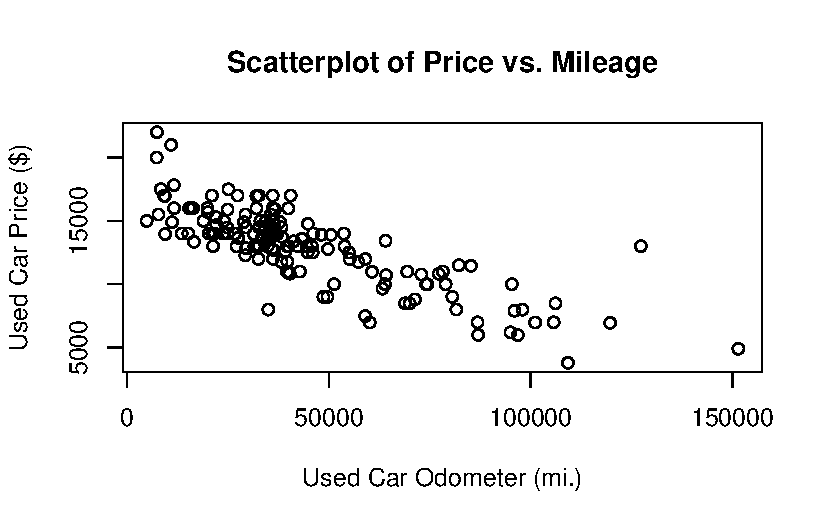
\includegraphics{Unidad1-resumen_files/figure-pdf/unnamed-chunk-60-1.pdf}

}

\end{figure}

Dando como resultado un gráfico similar a:

\begin{figure}

{\centering 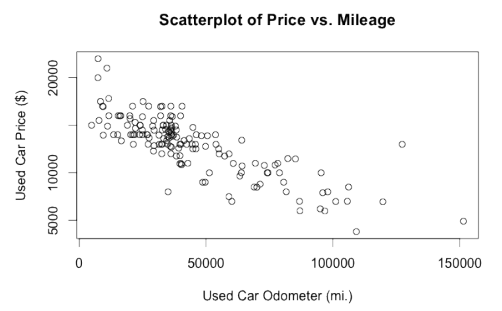
\includegraphics{dispersion.png}

}

\caption{Diagrama de dispersión}

\end{figure}

Si analizamos el diagrama se puede observar como cambian los valores de
la variable del eje y a medida que aumentan los valores del eje x.

\hypertarget{examen-de-las-relaciones-tabulaciones-cruzadas-de-dos-factores}{%
\paragraph{Examen de las relaciones: tabulaciones cruzadas de dos
factores}\label{examen-de-las-relaciones-tabulaciones-cruzadas-de-dos-factores}}

Para examinar una relación entre dos variables nominales, se utiliza una
tabulación cruzada bidireccional la cual es similar a un diagrama de
dispersión en el sentido de que permite examinar cómo cambian los
valores de una variable en función de los valores de otra. El formato es
una tabla en la que las filas son los niveles de una de una variable y
las columnas son los niveles de otra.

Como se sabe existen varias funciones para crear una tabla en R, una de
las funciones más facil de usar es CrossTable( ) del paquete gmodels
debido a que presenta los porcentajes de fila, columna en una sola
tabla, facilitando el proceso. Para instalar este paquete se utiliza:

\begin{Shaded}
\begin{Highlighting}[]
\CommentTok{\#install.packages("gmodels")}
\end{Highlighting}
\end{Shaded}

Posterior a esto se debe cargar el paquete con la función
library(gmodels).

Para continuar con el análisis, simplificaremos los niveles de la
variable color, para esto se dividirá los colores en 2 grupos creando
una variable indicadora binaria (variable ficticia), que indica el color
del coche, si es un color conservador según nuestra definición su valor
será 1 (verdadero) y 0 si no lo es.

\begin{Shaded}
\begin{Highlighting}[]
\NormalTok{usedcars}\SpecialCharTok{$}\NormalTok{conservative }\OtherTok{\textless{}{-}}\NormalTok{ usedcars}\SpecialCharTok{$}\NormalTok{color }\SpecialCharTok{\%in\%} \FunctionTok{c}\NormalTok{(}\StringTok{"Black"}\NormalTok{, }\StringTok{"Gray"}\NormalTok{, }\StringTok{"Silver"}\NormalTok{, }\StringTok{"White"}\NormalTok{)}
\end{Highlighting}
\end{Shaded}

Dentro de la función antes mencionada se debe mencionar que el comando
\%in\% regresa verdadero o falso para cada valor en el vector. Para
examinar los resultados de nuestra tabla creada podemos utilizar el
comando:

\begin{Shaded}
\begin{Highlighting}[]
\FunctionTok{table}\NormalTok{(usedcars}\SpecialCharTok{$}\NormalTok{conservative)}
\end{Highlighting}
\end{Shaded}

\begin{verbatim}

FALSE  TRUE 
   51    99 
\end{verbatim}

Al ver una tabulación cruzada se puede observar como varía la proporción
de color conservador según el modelo. Utilizaremos el comando
CrossTable( ):

\begin{Shaded}
\begin{Highlighting}[]
\CommentTok{\#CrossTable(x = usedcars$model, y = usedcars$conservative)}
\end{Highlighting}
\end{Shaded}




\end{document}
